%%
%% Commands for TeXCount
%TC:macro \cite [option:text,text]
%TC:macro \citep [option:text,text]
%TC:macro \citet [option:text,text]
%TC:envir table 0 1
%TC:envir table* 0 1
%TC:envir tabular [ignore] word
%TC:envir displaymath 0 word
%TC:envir math 0 word
%TC:envir comment 0 0

%%
%% For anonymous submission (double-blind review), use:
\PassOptionsToPackage{table}{xcolor}
\documentclass[sigconf,anonymous,review,9pt]{acmart}

%%
\AtBeginDocument{%
  \providecommand\BibTeX{{%
    Bib\TeX}}}

%%
\setcopyright{acmlicensed}
\copyrightyear{2026}
\acmYear{2026}
\acmDOI{XXXXXXX.XXXXXXX}
\acmConference[ICCAD'26]{IEEE/ACM International Conference on Computer-Aided Design}{November 8--12, 2026}{San Jose, CA, USA}
\acmISBN{978-1-4503-XXXX-X/26/11}

%%
\usepackage{amsmath,amsfonts}
\usepackage{multirow}
\usepackage{algorithm}
\usepackage{algorithmic}
\usepackage{booktabs}
\usepackage{subcaption}
\usepackage{url}
\definecolor{posstrong}{HTML}{C6EFCE}   % green – strong positive rho
\definecolor{posweak}{HTML}{E2EFDA}     % light green – moderate positive
\definecolor{neutral}{HTML}{F2F2F2}     % grey – near-zero rho
\definecolor{negweak}{HTML}{FDE8E8}     % pink – negative rho
\definecolor{rankfirst}{HTML}{FFCCCC}   % light red – best
\definecolor{ranksecond}{HTML}{CCE5FF}  % light blue – second best

\usepackage{caption}
\captionsetup{font=small}

\newcommand{\tpm}{$\pm$}

\begin{document}

\title{PPAPlace: Differentiable Cross-Stage Objectives for Chip Placement Optimization}

\author{Ruogu Chen}
\affiliation{%
  \institution{University of Alberta}
  \department{Department of Electrical and Computer Engineering}
  \city{Edmonton}
  \state{AB}
  \country{Canada}
}
\email{ruogu@ualberta.ca}

\author{Jie Han}
\affiliation{%
  \institution{University of Alberta}
  \department{Department of Electrical and Computer Engineering}
  \city{Edmonton}
  \state{AB}
  \country{Canada}
}
\email{jhan8@ualberta.ca}

%% ============================================================
\begin{abstract}
Macro placement significantly affects the chip's post-route performance,
power, and area (PPA). Most placement methods optimize half-perimeter wirelength
(HPWL) as the primary objective. However, recent benchmarking shows a near-zero correlation between HPWL and post-route timing metrics such as worst negative slack (WNS) and total negative slack (TNS). As a result, all evaluated artificial-intelligence (AI)-based placers in this benchmarking degrade PPA relative to a hierarchical baseline placer. Recent efforts have tried to train cross-stage predictors to close this gap. However, existing methods focus on macro-only representations and use pre-route metrics as training labels. This work conducts a training label fidelity study across ten circuits and four design flow stages, revealing that HPWL and pre-route timing are uninformative for predicting the final PPA. In contrast, post-global-routing achieves the best balance between final PPA fidelity and label generation cost-effectiveness. Based on this finding, this work proposes PPAPlace, a differentiable surrogate that predicts post-route PPA from the full mixed-size placement state. The surrogate is a dual-stream predictor that combines graph attention over the chip netlist with spatial convolution over the placement grid. It is trained on post-global-routing labels. The gradients of $\text{PPA}$ with respect to placement $\text{position}$ flow end-to-end from predicted PPA back to cell coordinates. PPAPlace exploits these gradients in two ways: as a co-objective injected into a differentiable analytical placer's analytical loop (PPAPlace-CoOpt), and as a post-placement refinement
step that adjusts macro positions via projected gradient descent (PPAPlace-Refine). On five unseen ChiPBench circuits, PPAPlace improves average WNS and TNS by 22\% and 51\% over the hierarchical baseline, and the predictor transfers across unseen circuits without retraining. Code is available at \url{https://anonymous.4open.science/r/PPAPlace}.
\end{abstract}

\keywords{chip placement, PPA prediction, differentiable objectives, surrogate-guided optimization, graph attention network, physical design}

\maketitle

%% ============================================================
\section{Introduction}
\label{sec:intro}

Chip placement determines the physical locations of circuit modules on a
two-dimensional canvas and is one of the most significant steps in very-large-scale integration physical design. The quality of placement directly affects the
chip's final performance, power consumption, and area (PPA), which
together determine whether a design meets its specifications for manufacturing~\cite{kahng2022vlsi}.

Existing placement approaches fall into two broad categories: analytical and artificial-intelligence (AI)-based placers. Analytical
placers such as DREAMPlace~\cite{lin2019dreamplace} formulate placement
as continuous optimization of a smooth wirelength approximation plus
density penalties, solved by gradient descent on a graphics processing unit (GPU). AI-based methods
including reinforcement
learning (RL)~\cite{mirhoseini2021graph, lai2022maskplace, lai2023chipformer},
black-box optimization~\cite{shi2023wire}, and diffusion
models~\cite{lee2024chip} replace or augment the optimizer with learned
policies. Despite the methodological differences between these two categories, most methods optimize the half-perimeter wirelength (HPWL), a fast estimate of total wire length, as the primary objective.

However, growing evidence suggests that HPWL is not as reliable a proxy as commonly assumed. The ChiPBench benchmark~\cite{chipbench2025} evaluated six AI-based placement methods on 20 circuits through the full
OpenROAD~\cite{ajayi2019openroad} chip design flow. It uses
Hier-RTLMP (Hierarchical Register-Transfer-Level Macro Placer), OpenROAD's built-in macro placer, as the baseline placement method. Hier-RTLMP leverages RTL design hierarchy and dataflow
structure rather than optimizing wirelength alone. The results show that every evaluated AI
method in ChiPBench degraded PPA relative to it. ChiPBench further reported a Pearson
correlation of only $-0.08$ between macro HPWL and the worst negative slack
(WNS), confirming that wirelength optimization is essentially
uninformative for timing.

Recent efforts have begun to close this gap from two
directions. AutoDMP~\cite{autodmp2023} tunes DREAMPlace's configuration
parameters through multi-objective Bayesian optimization (BO). It
uses post-placement proxies such as rectilinear Steiner minimum tree
(RSMT) wirelength, cell density, and rectangular uniform wire density
(RUDY) congestion to guide the search. While effective at improving placement
diversity, these proxies are computed before routing and suffer a similar
proxy-to-PPA gap. Therefore, they do not always stay faithful to the post-route PPA.
LaMPlace~\cite{lamplace2025} takes a complementary approach. It trains a
cross-stage predictor on offline placement data and uses it to guide
macro placement through evolutionary search, achieving notable timing
improvements. While these methods confirm that cross-stage prediction
is a viable path to better placement, they share two
unexamined assumptions. First, they adopt pre-route static timing analysis (STA)
as supervision data without verifying that such labels faithfully
preserve post-route PPA information. Second, existing methods represent the placement through macro positions alone, discarding the standard cell density
and routing congestion that ultimately govern timing and power.

This paper evaluates both assumptions. A controlled study across ten ChiPBench circuits reveals that pre-route timing labels, which were used as supervision data in prior works, can be misleading. Post-global-routing (GRT) labels, by contrast, consistently achieve high fidelity with final sign-off PPA and remain cost-effective in generation. This finding establishes a principled basis for selecting the supervision stage in any future cross-stage learning approach.

Built on this finding, this paper proposes PPAPlace, the first
differentiable cross-stage surrogate that estimates post-route PPA
from the complete mixed-size placement state. A dual-stream predictor
is trained on post-GRT labels. The graph attention stream encodes
netlist connectivity. The spatial convolution stream encodes cell
density, pin density, and RUDY congestion. Every component operates
within a differentiable computation graph, enabling end-to-end
gradient flow from predicted PPA back to cell coordinates.

Because the surrogate is fully differentiable, it provides not only
PPA predictions but also gradients
$\partial\text{PPA}/\partial\text{position}$ that indicate how moving
each cell would affect post-route timing. These gradients can be
injected directly into a differentiable placer's optimization loop as a
learned co-objective, complementing wirelength and density with
routing-aware PPA feedback. The same predictor also supports post-placement gradient descent to locally refine any converged placement, offering placer-agnostic
applicability.

The novel contributions are as follows:

\begin{enumerate}
    \item A label fidelity study across ten circuits and four design
    stages, establishing post-global-routing as the most
    cost-effective supervision stage for cross-stage PPA prediction.

    \item A differentiable dual-stream predictor over the complete
    mixed-size placement state, with end-to-end gradient flow from
    predicted PPA back to cell positions. It achieves nearly
    $4\times$ higher ranking accuracy than the macro-only, pre-route
    paradigm.

    \item Two gradient-guided deployment modes. PPAPlace-CoOpt
    injects the surrogate as a co-objective into DREAMPlace's
    analytical loop for global topology guidance. PPAPlace-Refine
    applies post-placement gradient descent to any converged
    placement for placer-agnostic local refinement. Combined, they
    improve WNS by 22\% and total negative slack (TNS) by 51\% over the hierarchical
    baseline, outperforming all evaluated prior methods.
\end{enumerate}

%% ============================================================
\section{Related Work}
\label{sec:related}

\begin{table*}[t]
    \centering
    \caption{Spearman $\rho_{\text{WNS}}$ between intermediate and post-route timing across ten training circuits (macro count in parentheses).
    \colorbox{posstrong}{Green}: $\rho \geq 0.7$;
    \colorbox{posweak}{light}: $0.3 \leq \rho < 0.7$;
    \colorbox{negweak}{pink}: negative. $\rho_{\text{TNS}}$ follows the same pattern.
    Rightmost column: average wall-clock cost of generating one label at each stage, shown on a \colorbox[HTML]{9EC1E4}{blue} scale to distinguish it from correlation.
    CTS: clock-tree synthesis; DRT: detailed routing.
    Post-DRT is the correlation reference ($\rho \equiv 1$, $3.7$\,hrs on average).}
    \label{tab:rank_corr}
    \renewcommand{\arraystretch}{1.15}
    \footnotesize
    \setlength{\tabcolsep}{5pt}
    \begin{tabular}{@{}l ccccc ccccc c @{\hspace{8pt}} c@{}}
    \toprule
    Stage
    & bp\_be & bp\_fe & bp\_be12 & isa\_npu & swerv
    & vga\_lcd & ether & dft68 & mor1kx & ari133
    & \textbf{Avg} & \textbf{Time} \\
    & \scriptsize(10) & \scriptsize(11) & \scriptsize(12)
    & \scriptsize(15) & \scriptsize(28) & \scriptsize(62)
    & \scriptsize(64) & \scriptsize(68) & \scriptsize(78)
    & \scriptsize(132) & & \scriptsize(hrs) \\
    \midrule
    HPWL
    & \cellcolor{neutral}+.12 & \cellcolor{negweak}$-.15$
    & \cellcolor{neutral}+.08 & \cellcolor{negweak}$-.21$
    & \cellcolor{neutral}+.05 & \cellcolor{negweak}$-.18$
    & \cellcolor{negweak}$-.09$ & \cellcolor{neutral}+.14
    & \cellcolor{negweak}$-.11$ & \cellcolor{neutral}+.03
    & \cellcolor{negweak}$-.03$
    & \cellcolor[HTML]{EAF2FB}$<$0.01 \\
    Pre-CTS STA
    & \cellcolor{neutral}+.15 & \cellcolor{neutral}+.09
    & \cellcolor{negweak}$-.07$ & \cellcolor{neutral}+.18
    & \cellcolor{negweak}$-.11$ & \cellcolor{neutral}+.06
    & \cellcolor{negweak}$-.14$ & \cellcolor{neutral}+.22
    & \cellcolor{neutral}+.03 & \cellcolor{neutral}+.12
    & \cellcolor{neutral}+.05
    & \cellcolor[HTML]{CDDFF2}0.08 \\
    Post-CTS
    & \cellcolor{posstrong}.83 & \cellcolor{posweak}.64
    & \cellcolor{posstrong}.71 & \cellcolor{posweak}.38
    & \cellcolor{negweak}$-.12$ & \cellcolor{neutral}.25
    & \cellcolor{negweak}$-.31$ & \cellcolor{posweak}.47
    & \cellcolor{neutral}.19 & \cellcolor{posstrong}.77
    & \cellcolor{posweak}.38
    & \cellcolor[HTML]{9EC1E4}0.14 \\
    \rowcolor{posstrong}
    \textbf{Post-GRT}
    & \textbf{.80} & \textbf{.91} & \textbf{.87} & \textbf{.85}
    & \textbf{.89} & \textbf{.82} & \textbf{.78} & \textbf{.84}
    & \textbf{.86} & \textbf{.94}
    & \textbf{.86}
    & \cellcolor[HTML]{6FA3D6}\textbf{0.20} \\
    \bottomrule
    \end{tabular}
    \renewcommand{\arraystretch}{1.0}
\end{table*}

\paragraph{Analytical placement}
Analytical placers formulate placement as continuous optimization of a
smooth wirelength objective subject to density
constraints~\cite{lu2015eplace, cheng2019replace}.
DREAMPlace~\cite{lin2019dreamplace} recast this formulation as a
neural network training problem, achieving over $30\times$ GPU
speedup. DREAMPlace~4.0~\cite{dreamplace4} added timing-driven net
weighting from pre-route STA. AutoDMP~\cite{autodmp2023} tunes 16
DREAMPlace parameters via multi-objective Tree-structured Parzen
Estimator using post-placement proxies (RSMT wirelength, cell
density, RUDY congestion) as BO objectives.

\paragraph{Differentiable placement objectives}
Recent work has extended gradient-based placement beyond wirelength
and density. Efficient-TDP~\cite{efficienttdp2025}
injects pin-to-pin attraction on critical paths into DREAMPlace using
pre-route STA, achieving state-of-the-art timing-driven standard-cell
placement. RoutePlacer~\cite{routeplacer2024} trains a graph neural
network on global-router overflow labels and injects the learned
congestion penalty as a differentiable objective into DREAMPlace's
loop, reducing routing overflow by up to 16\%.
These methods each target a single intermediate metric such as
pre-route timing or routability. None addresses mixed-size placement
or post-route PPA as the optimization objective.

\paragraph{AI-based placement}
AlphaChip~\cite{mirhoseini2021graph} pioneered deep reinforcement
learning for macro placement, though its reproducibility remains
debated~\cite{kahng2023reevaluating}. Subsequent work explored visual
representation learning~\cite{lai2022maskplace}, offline
RL~\cite{lai2023chipformer}, evolutionary
search~\cite{shi2023wire}, placement
refinement~\cite{maskregulate2024}, and tree-search-guided
RL~\cite{efficientplace2024}. All optimize HPWL or macro HPWL as the
primary objective.

\paragraph{Cross-stage PPA prediction and optimization}
LaMPlace~\cite{lamplace2025} trains a Laurent polynomial predictor to
estimate cross-stage metrics from macro pairwise distances and uses it
to guide WireMask-EA's evolutionary search. Its training labels come
from OpenTimer placement-based STA, which estimates wire delays from
coordinates alone and assumes ideal clocks.
MacroRank~\cite{macrorank2023} and
PreRoutGNN~\cite{preroutgnn2024} predicted placement or routing
quality but did not use predictions to improve placement.
Re$^2$MaP~\cite{re2map2025} achieves state-of-the-art macro placement
through recursive prototyping and packing-tree relocation with
hand-engineered cost terms. It represents the best of algorithmic
macro placement but does not use learned objectives.
BBOPlace-Bench~\cite{bboplacebench2025} benchmarks black-box
optimization approaches to macro placement. It argues for aligning
the search objective with downstream PPA. In the commercial space,
Synopsys DSO.ai~\cite{dsoai2025} and Cadence
Cerebrus~\cite{cerebrus2025} use reinforcement learning to tune tool
configurations across the design flow, treating placement as part of
a broader design-space optimization problem. Across these efforts, no
work has systematically validated which design flow stage provides the
most reliable supervision for cross-stage prediction.


%% ============================================================
\section{Preliminaries}
\label{sec:prelim}

\subsection{Chip Placement and Evaluation Metrics}

Chip placement assigns physical positions to circuit modules on a
two-dimensional canvas. A netlist hypergraph $H = (V, E)$ specifies the
modules $V$ (macros and standard cells) and the nets $E$ connecting
them. Placement methods seek positions
$\mathbf{x} = \{(x_i, y_i)\}_{i=1}^{N}$ that minimize a placement
objective. In analytical placers such as
DREAMPlace~\cite{lin2019dreamplace}, this takes the form:
\begin{equation}
\label{eq:placement}
\min_{\mathbf{x}} \; \mathcal{L}(\mathbf{x})
= \mathcal{W}(\mathbf{x}) + \lambda \cdot \mathcal{D}(\mathbf{x}),
\end{equation}
where $\mathcal{W}$ is a smooth wirelength approximation and
$\mathcal{D}$ is a density penalty that discourages cell
overlap~\cite{lu2015eplace}. The density weight $\lambda$ increases
iteratively to enforce legality. The wirelength term is typically based
on HPWL:
\begin{equation}
\label{eq:hpwl}
\mathrm{HPWL}(\mathbf{x}) = \sum_{e \in E}
\left[\max_{i \in e} x_i - \min_{i \in e} x_i
+ \max_{i \in e} y_i - \min_{i \in e} y_i\right],
\end{equation}
which estimates total wire length by summing the bounding-box
half-perimeters across all nets. HPWL is differentiable (via smooth
approximations such as the weighted-average
model~\cite{hsu2013wa}), decomposable across nets, and fast to compute.

However, the actual quality of a placed design is determined by
post-route PPA metrics obtained after executing the downstream flow:
clock tree synthesis (CTS), global routing (GRT), and detailed routing
(DRT), each adding fidelity to timing and congestion estimates. Let
$\mathrm{Flow}(\mathbf{x})$ denote the full flow and
$\mathrm{Flow}_s(\mathbf{x})$ denote the flow truncated at stage $s$:
\begin{equation}
\label{eq:ppa}
\mathbf{y} = \mathrm{Flow}(\mathbf{x})
= \left[\mathrm{WNS},\; \mathrm{TNS},\;
\mathrm{Power},\; \mathrm{Area}\right],
\end{equation}
\begin{equation}
\label{eq:partial_flow}
\mathbf{y}_s = \mathrm{Flow}_s(\mathbf{x}), \quad
s \in \{\text{CTS},\; \text{GRT},\; \text{DRT}\},
\end{equation}
where WNS is the worst negative slack, TNS is the total negative slack,
and power and area are the total power consumption and physical footprint.
Computing $\mathbf{y}$ typically takes tens of minutes to hours.

The goal of a cross-stage PPA predictor is to learn
$f_\theta(\mathbf{x}) \approx \mathbf{y}_{\text{DRT}}$ from
placement-stage features, thus avoiding the cost of running
$\mathrm{Flow}(\mathbf{x})$ at inference time. A prerequisite is that
the training labels $\mathbf{y}_s$ used to supervise $f_\theta$ must
rank placements of different quality consistently with the final outcome
$\mathbf{y}_{\text{DRT}}$.
Section~\ref{sec:label_fidelity} investigates which stage $s$ best
satisfies this requirement.

%% ============================================================
\section{Label Fidelity Analysis}
\label{sec:label_fidelity}

\begin{figure*}[t]
    \centering
    
\includegraphics[width=\textwidth]{graphs/ppaplace_overview.pdf}
    \caption{PPAPlace framework.
    (a)~Offline training on post-GRT labels.
    (b)~CoOpt: surrogate gradients injected into DREAMPlace as a co-objective.
    (c)~Refine: post-placement gradient descent on the converged result.}
    \label{fig:overview}
\end{figure*}

\subsection{Setup}

This study spans 10 ChiPBench~\cite{chipbench2025} circuits covering
RISC-V CPUs from three families (bp\_fe, bp\_be, and bp\_be12 from
BlackParrot, swerv\_wrapper from SweRV, ariane133 from Ariane), an
OpenRISC CPU (mor1kx), a neural processing unit (isa\_npu), and
peripheral designs (ethernet, dft68, vga\_lcd). The number of macros ranges from 10 to 132 and cell counts from 33K to 427K,
ensuring that the findings are not specific to a single design scale
or application domain. Note that this fidelity test uses RTLMP weight
configurations evaluated through the full flow, and is independent of
the training/test split used for the main experiments in
Section~\ref{sec:experiments}.

To generate diverse placements for each circuit, the weight parameters
of OpenROAD's RTLMP hierarchical macro
placer~\cite{ajayi2019openroad} are systematically varied. RTLMP
optimizes a weighted combination of six objectives controlled by
\textsc{area\_wt}, \textsc{wirelength\_wt}, \textsc{boundary\_wt},
\textsc{outline\_wt}, \textsc{notch\_wt}, and \textsc{dead\_space}.
For each circuit, 20 configurations are evaluated:
1~default (all weights at their ChiPBench defaults),
12~single-parameter sweeps (each of the six weights set to a high
value of $20$ or a low value of $0.1$, with all others at default),
and 7~multi-parameter combinations that probe pairwise interactions
(e.g., area$+$wirelength both at $10$, wirelength$+$boundary both at $10$)
and global extremes (all three main weights at $10$ or at $0.1$).
Because RTLMP is deterministic given a weight configuration, each
of the 20 settings produces exactly one placement per circuit,
yielding 200 unique placements across the 10 circuits.

Each configuration is evaluated through the complete ChiPBench flow:
synthesis, floorplanning with the specified RTLMP weights, standard cell
placement, CTS, GRT, and DRT. PPA metrics (WNS, TNS, power) are
recorded at each stage. Area is excluded because it is determined by the
floorplan and remains constant across different placements for the same circuit.
Because the entire flow runs within a single ChiPBench pipeline, all
stages share the same synthesized netlist and extracted parasitics,
ensuring internal consistency across stages. Post-DRT metrics serve as
the ground truth throughout this analysis.

\subsection{Stage-Wise Rank Correlation}

Table~\ref{tab:rank_corr} reports Spearman $\rho_{\text{WNS}}$ between
each intermediate stage and the post-route ground truth. WNS and TNS
show the same pattern. Only WNS is reported. 

HPWL has near-zero
average correlation ($\bar\rho = -0.03$), with negative values on 5 of
10 circuits. Pre-CTS STA, the label source used by
LaMPlace~\cite{lamplace2025}, is similarly uninformative
($\bar\rho = +0.05$). Post-CTS is inconsistent: strongly positive on
some circuits (bp\_be: $\rho = 0.83$) but negative on others
(ethernet: $\rho = -0.31$). Post-GRT achieves $\rho \geq 0.78$ on all
10 circuits with no sign reversals ($\bar\rho = 0.86$). It costs
$0.20$\,hrs per sample on average versus $3.7$\,hrs for full DRT
(Table~\ref{tab:rank_corr}). It is thus the most cost-effective
supervision stage.


%% ============================================================
\section{PPAPlace}
\label{sec:method}

Based on the findings in Section~\ref{sec:label_fidelity}, PPAPlace
uses post-global-routing labels as training supervision. PPAPlace
has three components. A differentiable PPA predictor is trained on the
mixed-size placement state
(Sections~\ref{subsec:representation}--\ref{subsec:training}). A
differentiable feature extraction layer enables gradient flow from
predictions back to cell positions
(Section~\ref{subsec:diff_features}). Two gradient-guided deployment
modes, co-objective placement and post-placement refinement, exploit
these gradients to improve placement quality
(Section~\ref{subsec:gradient_placement}).
Figure~\ref{fig:overview} illustrates the overall design.


\subsection{Mixed-Size Placement Representation}
\label{subsec:representation}

Existing cross-stage predictors such as LaMPlace~\cite{lamplace2025} represent the
placement state through macro pairwise distances, discarding information
about standard cells, spatial density, and routing congestion. However,
timing violations and power consumption are largely affected by
standard cell placement and routing, not macro positions
alone~\cite{chipbench2025}. PPAPlace addresses this by observing the
complete mixed-size placement through two complementary representations.

\textbf{Spatial representation.} The placement canvas is rasterized into
a $64 \times 64$ grid with five channels:
\begin{enumerate}
    \item Cell density: total cell area overlapping each bin,
    normalized by bin capacity.
    \item Pin density: I/O pin concentration per bin.
    \item Macro occupancy: degree of macro presence in each bin.
    \item RUDY congestion: estimated routing demand per
    bin~\cite{rudy}, computed as $\sum_{e} 1/(W_e \cdot H_e)$ over
    nets $e$ whose bounding box overlaps the bin, where $W_e$ and $H_e$
    are bounding box dimensions.
    \item Net bounding box density: net bounding box overlap
    per bin, capturing routing pressure from nets whose
    pins lie outside the bin.
\end{enumerate}
All channels are normalized to $[0, 1]$. This grid-based representation
captures spatial distribution patterns invisible to macro-only
predictors, including congestion hotspots and density imbalances.

\textbf{Graph representation.} The netlist is represented as a graph
$G = (V_G, E_G)$ where macros are the nodes. Edges are derived
from the netlist hypergraph: each multi-pin net connecting $k$ macros
produces $\binom{k}{2}$ undirected edges (clique expansion), with
duplicate edges merged and edge weights set to the number of shared
nets between each macro pair. Each node carries
a feature vector:
\begin{equation}
\label{eq:node_features}
\mathbf{h}_i = [x_i,\; y_i,\; w_i,\; h_i,\; r_i,\; p_i,\;
n_i,\; s_i],
\end{equation}
where $(x_i, y_i)$ is normalized position, $(w_i, h_i)$ is normalized
width and height, $r_i = w_i / h_i$ is aspect ratio, $p_i$ is pin
count, $n_i$ is net degree (number of nets connected to this node), and
$s_i$ is average net span (mean HPWL of connected nets). 

The two streams are complementary: the spatial grid captures global density and routing pressure while the graph captures per-macro identity and local connectivity.

\subsection{Dual-Stream PPA Predictor}
\label{subsec:architecture}

The two representations are processed by separate encoder streams and
fused for prediction.

\textbf{Spatial stream.} A lightweight convolutional neural network (CNN) with 3 layers
and ReLU activations progressively reduces the spatial
resolution of the $64 \times 64$ grid. Global average
pooling (GAP) produces
a spatial embedding $\mathbf{e}_s \in \mathbb{R}^{256}$.

\textbf{Graph stream.} A 4-layer graph attention network
(GAT)~\cite{gat2018} with 128-dimensional hidden states and 4
attention heads processes the netlist graph. Multi-head attention allows
each layer to learn different types of relationships between connected
nodes, such as spatial proximity and connectivity strength. GAP aggregates all node embeddings into a fixed-size graph embedding
$\mathbf{e}_g \in \mathbb{R}^{256}$, regardless of circuit size.

\textbf{Fusion and prediction.} The two embeddings are concatenated and
mapped to PPA predictions through a 2-layer multi-layer perceptron (MLP):
\begin{equation}
\label{eq:predictor}
f_\theta(\mathbf{x}) =
\mathrm{MLP}\!\left([\mathbf{e}_g(\mathbf{x});\;
\mathbf{e}_s(\mathbf{x})]\right) \rightarrow
[\widehat{\mathrm{WNS}},\; \widehat{\mathrm{TNS}},\;
\widehat{\mathrm{Power}},\; \widehat{\mathrm{Area}}].
\end{equation}
The hat notation denotes predicted values. The architecture produces
fixed-size embeddings (512 dimensions total) regardless of circuit size,
enabling the same trained model to be applied across circuits with
different numbers of cells and macros. Because the entire pipeline (feature extraction, GAT, CNN, MLP) is composed of differentiable operations, the Jacobian $\partial f_\theta / \partial \mathbf{p}$, where $\mathbf{p}$ is the vector of cell positions, is available via automatic differentiation. This Jacobian indicates how each cell's position influences predicted post-route PPA.


\subsection{Training}
\label{subsec:training}

\subsubsection{Data Generation}

Training data is generated by running a placement method with $M$
randomized configurations per circuit. Each configuration varies
parameters that affect placement quality, such as target density and
density weight schedule. As discussed in Section~\ref{sec:label_fidelity}, each resulting placement is
evaluated through the OpenROAD flow to post-global-routing, producing
labels $\mathbf{y}_i = [\mathrm{WNS},\; \mathrm{TNS},\;
\mathrm{Power},\; \mathrm{Area}]$. The training set is
$\mathcal{D} = \{(\mathbf{x}_i, \mathbf{y}_i)\}_{i=1}^{C \times M}$
across $C$ circuits.

\subsubsection{Loss Function}

The predictor is trained with a composite loss:
\begin{equation}
\label{eq:loss}
\mathcal{L} = \mathcal{L}_{\mathrm{MSE}}
+ \lambda_r \cdot \mathcal{L}_{\mathrm{rank}}.
\end{equation}
$\mathcal{L}_{\mathrm{MSE}}$ is the mean squared error between
predicted and true PPA values. However, the core task of the predictor is not to estimate exact PPA values,
but to correctly rank which placements produce superior PPA and which produce inferior PPA.
Because of this, $\mathcal{L}_{\mathrm{rank}}$ is a pairwise ranking loss
computed over placement pairs from the same circuit:
\begin{equation}
\label{eq:ranking}
\mathcal{L}_{\mathrm{rank}} = \sum_{(i,j)}
\max\!\Big(0,\; -(\mathbf{y}_i - \mathbf{y}_j) \cdot
\big(f_\theta(\mathbf{x}_i) - f_\theta(\mathbf{x}_j)\big)\Big),
\end{equation}
where the sum is over all placement pairs $(i, j)$ from the same
circuit. All four PPA metrics are sign-unified (lower is better) and
z-score normalized per circuit. The hinge incurs zero loss for
correctly ranked pairs and a linear penalty for misranked ones,
directly optimizing ordinal accuracy. Power varies by less than 2\%
across configurations of the same circuit, so timing dominates the
ranking signal. With $M = 500$ samples per circuit, each mini-batch
covers $\binom{500}{2} \approx 125$K pairs per epoch.
The MSE term stabilizes learning with an absolute signal, while
the ranking loss optimizes the ordinal accuracy needed for deployment.

\subsection{Differentiable Feature Extraction}
\label{subsec:diff_features}

The feature extraction layer maps cell positions to the spatial grid
and node features of Section~\ref{subsec:representation} through
differentiable operations. This ensures that gradients
$\partial f_\theta / \partial \mathbf{p}$ flow end-to-end from
predicted PPA back to cell coordinates. The same differentiable
features are used during both training and gradient-guided placement.

\textbf{Spatial channels.} Each of the five channels is computed as a
continuous function of cell positions. Cell density (channel~0) uses
clamp-based overlap area. This is piecewise linear and differentiable
almost everywhere, matching the functional form DREAMPlace uses for
its density penalty. Pin density (channel~1) uses Gaussian splatting
($\sigma = 1.5$ bin widths), distributing each pin's contribution
smoothly across neighboring bins. Macro occupancy (channel~2) uses
sigmoid soft masks ($\sigma = 20$), producing a near-binary mask with
a smooth transition at macro boundaries. RUDY congestion (channel~3)
computes net bounding boxes via the log-sum-exp smooth approximation
to $\max$ and $\min$ (temperature $\gamma = 10$), matching
DREAMPlace's wirelength smoothing. Net bounding-box density
(channel~4) uses the same Gaussian splatting as channel~1.

\textbf{Node features.} Positions $x_i, y_i$ enter the feature vector
(Eq.~\ref{eq:node_features}) directly. Average net span $s_i$ uses
the same log-sum-exp HPWL approximation as the spatial RUDY channel.
Static features (width, height, pin count, net degree) carry zero
gradient and require no modification. Channel normalization uses
$\mathbf{g}_c / (\max(\mathbf{g}_c) + \epsilon)$, where $\max$ is
differentiable via PyTorch's \texttt{amax}.

The full pipeline from cell positions $\mathbf{p}$ through feature
extraction, GAT, CNN, and MLP to predicted PPA is end-to-end
differentiable by construction. The gradient
$\nabla_{\mathbf{p}} f_\theta$ is available via a single backward
pass.


\subsection{Gradient-Guided Placement}
\label{subsec:gradient_placement}

Given the differentiable surrogate $f_\theta$ and a placement \\
$\mathbf{p} = (x_1, y_1, \ldots, x_N, y_N)$, the gradient
$\nabla_{\mathbf{p}} f_\theta$ indicates how each cell's position
affects predicted post-route PPA. PPAPlace exploits this signal in two
complementary modes.

\textbf{Co-objective placement (PPAPlace-CoOpt).}
The surrogate is injected directly into DREAMPlace's analytical
placement loop as a third objective alongside wirelength and density
(Algorithm~\ref{alg:coopt}). DREAMPlace first runs $W$ warmup
iterations to reach a rough solution within the surrogate's training
distribution. The total objective then becomes:
\begin{equation}
\label{eq:coopt}
\mathcal{L}_{\mathrm{total}} = \mathcal{L}_{\mathrm{WL}}
  + \lambda_d\,\mathcal{L}_{\mathrm{density}}
  + \lambda_p\,(\widehat{\mathrm{WNS}} + \widehat{\mathrm{TNS}}),
\end{equation}
where $\widehat{\mathrm{WNS}}$ and $\widehat{\mathrm{TNS}}$ are the
timing outputs of $f_\theta(\mathbf{p})$ (power and area outputs are
unused, as they are insensitive to placement changes within the same
floorplan), and $\lambda_p$ increases linearly from 0 to its target value over
the remaining iterations. The gradient reaches macros through both
streams and standard cells through the spatial grid's pin-density,
RUDY, and net-bounding-box channels, so CoOpt reshapes standard-cell
clustering as well as macro placement, which no analytical proxy
achieves.

\begin{algorithm}[h]
\caption{PPAPlace-CoOpt: Co-Objective Placement}
\label{alg:coopt}
\footnotesize
\begin{algorithmic}[1]
\REQUIRE Predictor $f_\theta$, warmup $W$, target weight $\lambda_p^*$,
  total iterations $N$
\STATE Initialize positions $\mathbf{p}_0$ randomly
\FOR{$t = 1, \ldots, N$}
  \STATE $\mathcal{L} \leftarrow \mathcal{L}_{\mathrm{WL}}
    + \lambda_d\,\mathcal{L}_{\mathrm{density}}$
    \hfill\COMMENT{standard DREAMPlace}
  \IF{$t > W$}
    \STATE $\lambda_p \leftarrow \lambda_p^* \cdot (t - W) / (N - W)$
      \hfill\COMMENT{linear ramp}
    \STATE $\mathcal{L} \leftarrow \mathcal{L}
      + \lambda_p\,(\widehat{\mathrm{WNS}} + \widehat{\mathrm{TNS}})$
      \hfill\COMMENT{timing co-objective}
  \ENDIF
  \STATE $\mathbf{p}_t \leftarrow \mathbf{p}_{t-1}
    - \eta\,\nabla_{\mathbf{p}}\mathcal{L}$
    \hfill\COMMENT{GPU-accelerated update}
\ENDFOR
\STATE \textbf{return} placement $\mathbf{p}_N$
\end{algorithmic}
\end{algorithm}

\textbf{Post-placement refinement (PPAPlace-Refine).}
Starting from any converged placement $\mathbf{p}_0$, projected
gradient descent minimizes the surrogate timing objective
(Algorithm~\ref{alg:refine}):
\begin{equation}
\label{eq:refine}
\mathbf{p}_{t+1} = \Pi_\mathcal{C}\!\left(\mathbf{p}_t
  - \alpha\,\nabla_{\mathbf{p}}
  \big[\widehat{\mathrm{WNS}} + \widehat{\mathrm{TNS}}\big]\right),
\end{equation}
where $\alpha$ is the learning rate and $\Pi_\mathcal{C}$ clips to
the die bounding box. The refined macros are then legalized to resolve overlaps and enforce
boundary constraints, and standard cells are re-optimized
with macros fixed. Only the refined macro locations survive this
handoff, so Refine is effectively a macro-position method, whereas
CoOpt reshapes the full mixed-size placement.

The two modes serve different roles. CoOpt reshapes the global cell
topology during placement but requires integration with a specific
analytical placer. Refine adjusts positions locally after placement
but is placer-agnostic: it applies to any method that produces a
placement, including commercial tools whose internals are
inaccessible (Section~\ref{subsec:main_results}).

\begin{algorithm}[h]
\caption{PPAPlace-Refine: Post-Placement Refinement}
\label{alg:refine}
\footnotesize
\begin{algorithmic}[1]
\REQUIRE Converged placement $\mathbf{p}_0$, predictor $f_\theta$,
  learning rate $\alpha$, steps $T$
\FOR{$t = 1, \ldots, T$}
  \STATE Compute differentiable features from $\mathbf{p}_{t-1}$
  \STATE $\hat{\mathbf{y}} \leftarrow f_\theta(\text{features})$
  \hfill\COMMENT{surrogate prediction ($<$0.1\,s)}
  \STATE $\mathbf{g} \leftarrow \nabla_{\mathbf{p}}
    (\widehat{\mathrm{WNS}} + \widehat{\mathrm{TNS}})$
  \hfill\COMMENT{backprop}
  \STATE $\mathbf{p}_t \leftarrow \Pi_\mathcal{C}(\mathbf{p}_{t-1}
    - \alpha\,\mathbf{g})$
  \hfill\COMMENT{projected gradient step}
\ENDFOR
\STATE Legalize $\mathbf{p}_T$; re-optimize standard cells
\STATE \textbf{return} refined placement $\mathbf{p}_T$
\end{algorithmic}
\end{algorithm}




%% ============================================================
\section{Experiments and Results}
\label{sec:experiments}

\subsection{Setup}
\label{subsec:setup}

\subsubsection{Benchmarks}
Experiments use ChiPBench~\cite{chipbench2025} circuits with the
Nangate45 library. Ten circuits serve as training data (bp\_fe,
bp\_be12, isa\_npu, bp\_multi, or1200, swerv\_wrapper43, vga\_lcd,
ethernet, dft68, mor1kx). Five held-out circuits are used for
end-to-end evaluation (swerv\_wrapper, ariane133, black\_parrot,
bp\_be, ariane136). The test set matches
LaMPlace's~\cite{lamplace2025} ChiPBench evaluation, enabling
ratio-level comparison under the same Hier-RTLMP normalization. All
placements are evaluated through the full OpenROAD post-route flow,
yielding WNS (ps), TNS (ns), power (mW), and area ($\mu$m$^2$).

\subsubsection{Training}
Per training circuit, 1{,}000 DREAMPlace configurations are sampled
by randomizing 10 hyperparameters: target density
$\in [0.70, 0.90]$, density weight $\in [10^{-5}, 10^{-3}]$
(log-uniform), learning rate $\in [10^{-3}, 0.032]$ (log-uniform),
gamma $\in [2, 10]$, stop overflow
$\in \{0.05, 0.07, 0.10, 0.15\}$, wirelength model \\
$\in \{\text{weighted-average}, \text{log-sum-exp}\}$, global-placement iterations
$\in \{800, 1000, 1200, 1500\}$, macro halo $\in [0, 10]$ sites,
noise ratio $\in [0.01, 0.05]$, and random seed $\in [1, 10^5]$.
Roughly 65\% of sampled configurations yield valid placements
(DREAMPlace convergence and successful OpenROAD flow). The
first 500 successful placements per circuit are retained and
evaluated through the OpenROAD flow to post-GRT, producing 5{,}000
training pairs across ten circuits.

The surrogate is trained end-to-end on these pairs using the composite
loss from Eq.~\ref{eq:loss} with ranking loss weight
$\lambda_r = 0.5$. Within each mini-batch of 32 samples, placements
are grouped by circuit so that ranking pairs compare designs with the
same netlist. The Adam optimizer runs for 200 epochs with learning
rate $5 \times 10^{-4}$ and weight decay $10^{-5}$. All results
report mean $\pm$ std over 3 independent runs with different seeds.

The label fidelity study (Section~\ref{sec:label_fidelity}) uses
RTLMP placements, while training uses DREAMPlace placements. This
does not create a mismatch. The fidelity analysis concerns the
relationship between flow stages and PPA metrics, which is a property
of the design flow rather than any specific placer.
Section~\ref{subsec:generalization} validates this empirically.

\subsubsection{Baselines and methods}
Seven baselines represent the current landscape.
Hier-RTLMP~\cite{hierrtlmp2023} is OpenROAD's hierarchical macro
placer and serves as the ChiPBench reference (all metrics normalized
to 1.00). DREAMPlace~\cite{lin2019dreamplace} is the GPU-accelerated
analytical placer run with the default wirelength-and-density
configuration adopted by ChiPBench~\cite{chipbench2025}.
DREAMPlace\,4.0~\cite{dreamplace4} adds pre-route STA net weighting
via OpenTimer; we run the authors' open-source release with default parameters.
AutoDMP~\cite{autodmp2023} automates DREAMPlace hyperparameter tuning
via multi-objective Bayesian optimization.
MaskRegulate~\cite{maskregulate2024} refines macro placements using RL
with a regularity-based reward.
LaMPlace~\cite{lamplace2025} trains a cross-stage predictor on
pre-route STA labels and searches with WireMask-EA evolutionary
optimization.
Re$^2$MaP~\cite{re2map2025} uses recursive mixed-size prototyping
with hand-engineered cost terms.
LaMPlace results are from its published evaluation
(marked~$^\dagger$). DREAMPlace, AutoDMP, and MaskRegulate results
are from ChiPBench's end-to-end evaluation~\cite{chipbench2025}
(marked~$^\ddagger$). Re$^2$MaP ratios are computed from its
published results under the same OpenROAD flow (marked~$^\S$).

Three PPAPlace configurations are evaluated, all using the same
trained surrogate. PPAPlace-Refine (Algorithm~\ref{alg:refine})
applies $T{=}30$ projected gradient descent steps
($\alpha{=}0.001$) on predicted WNS$+$TNS to a DREAMPlace default
placement, followed by legalization and standard-cell re-optimization.
PPAPlace-CoOpt (Algorithm~\ref{alg:coopt}) injects the surrogate as a
co-objective into DREAMPlace's analytical loop. After $W{=}200$ warmup
iterations, the PPA loss weight $\lambda_p$ ramps linearly to $0.01$.
PPAPlace-CoOpt{+}Refine applies Refine after CoOpt, combining global
topology guidance with local gradient refinement.

\subsubsection{Hardware and offline cost}
All experiments run on a single NVIDIA RTX A6000 GPU (48\,GB) with an
Intel Xeon Gold 5218R CPU and 64\,GB RAM. DREAMPlace runs on GPU
(${\sim}$24\,s per configuration). Post-GRT evaluation runs on CPU
with 16 concurrent OpenROAD processes
($0.2$\,h per sample on average, ranging from ${\sim}0.05$\,h on the
smallest circuits to ${\sim}0.3$\,h on the largest; see
Table~\ref{tab:rank_corr}). Generating all 5{,}000 training labels
takes ${\sim}$63\,h wall-clock with placement and evaluation
pipelined. Model training takes ${\sim}$45\,min. This offline cost is
amortized: the same dataset and model serve all downstream experiments
without additional labeling.


\subsection{Main Results}
\label{subsec:main_results}

\begin{table*}[t]
\centering
\caption{Post-route timing normalized by Hier-RTLMP (lower is better). PPAPlace rows report mean $\pm$ std over 3 independently seeded runs; baselines are deterministic or from published results. \colorbox{rankfirst}{\textbf{Bold}}: best; \colorbox{ranksecond}{\underline{underline}}: second best.
$^\dagger$: from~\cite{lamplace2025}; $^\ddagger$: from ChiPBench~\cite{chipbench2025}; $^\S$: ratios computed from~\cite{re2map2025} (same OpenROAD flow; std-cell placement differs).}
\label{tab:main}
\footnotesize
\setlength{\tabcolsep}{4pt}
\resizebox{\textwidth}{!}{%
\begin{tabular}{@{}l@{\hskip 8pt}l cc cc cc cc cc ccc@{}}
\toprule
& & \multicolumn{2}{c}{swerv\_wrap}
& \multicolumn{2}{c}{ariane133}
& \multicolumn{2}{c}{black\_parrot}
& \multicolumn{2}{c}{bp\_be}
& \multicolumn{2}{c}{ariane136}
& \multicolumn{3}{c}{\textbf{Average}} \\
\cmidrule(lr){3-4}\cmidrule(lr){5-6}\cmidrule(lr){7-8}
\cmidrule(lr){9-10}\cmidrule(lr){11-12}\cmidrule(lr){13-15}
Method & Objective
  & WNS & TNS & WNS & TNS & WNS & TNS
  & WNS & TNS & WNS & TNS & WNS & TNS & Pwr \\
\midrule
\multicolumn{15}{@{}l}{\emph{Prior placement methods}} \\[1pt]
Hier-RTLMP~\cite{hierrtlmp2023} & hierarchy
  & 1.00 & 1.00 & 1.00 & 1.00 & 1.00 & 1.00
  & 1.00 & 1.00 & 1.00 & 1.00 & 1.00 & 1.00 & 1.00 \\
DREAMPlace$^\ddagger$~\cite{lin2019dreamplace} & HPWL
  & 1.13 & 0.93 & 2.90 & 0.61 & 0.94 & 1.82
  & 0.87 & 0.86 & 2.23 & 5.37 & 1.61 & 1.92 & 1.00 \\
DREAMPlace\,4.0~\cite{dreamplace4} & pre-route STA
  & 1.02 & 0.88 & 1.65 & 0.58 & 0.91 & 1.30
  & 0.82 & 0.83 & 1.45 & 2.85 & 1.17 & 1.29 & 1.01 \\
AutoDMP$^\ddagger$~\cite{autodmp2023} & config.\ tuning
  & 1.43 & 1.47 & 1.44 & 1.76 & 1.01 & 0.85
  & \cellcolor{rankfirst}\textbf{0.49} & 1.03 & 1.62 & 3.69 & 1.20 & 1.76 & 1.02 \\
MaskRegulate$^\ddagger$~\cite{maskregulate2024} & regularity
  & 1.02 & 0.84 & \cellcolor{rankfirst}\textbf{0.60} & \cellcolor{rankfirst}\textbf{0.24} & 0.91 & \cellcolor{ranksecond}\underline{0.14}
  & 0.85 & 0.83 & 1.67 & 3.42 & 1.01 & 1.09 & 1.00 \\
LaMPlace$^\dagger$~\cite{lamplace2025} & pre-route STA
  & 1.55 & 1.21 & 1.48 & 1.77 & 1.18 & 1.28
  & 1.25 & 1.38 & 1.12 & 1.15 & 1.32 & 1.36 & -- \\
Re$^2$MaP$^\S$~\cite{re2map2025} & heuristic
  & \cellcolor{ranksecond}\underline{0.78} & \cellcolor{ranksecond}\underline{0.62} & 0.93 & 0.99 & 0.98 & \cellcolor{rankfirst}\textbf{0.02}
  & 0.85 & \cellcolor{ranksecond}\underline{0.51} & 0.92 & 0.91 & 0.89 & 0.61 & 1.00 \\
\midrule
\multicolumn{15}{@{}l}{\emph{Gradient-guided placement (ours)}} \\[1pt]
PPAPlace-Refine & $\nabla$surrogate
  & 1.02\tpm.03 & 0.85\tpm.03
  & 2.15\tpm.08 & 0.52\tpm.04
  & 0.88\tpm.02 & 1.20\tpm.05
  & 0.78\tpm.02 & 0.72\tpm.04
  & 1.65\tpm.06 & 3.50\tpm.10
  & 1.30\tpm.04 & 1.36\tpm.05 & 1.01 \\
PPAPlace-CoOpt & $\nabla$surrogate
  & 0.82\tpm.03 & 0.68\tpm.04
  & 0.90\tpm.04 & 0.50\tpm.03
  & \cellcolor{ranksecond}\underline{0.84\tpm.02} & 0.22\tpm.04
  & 0.72\tpm.02 & 0.55\tpm.04
  & \cellcolor{ranksecond}\underline{0.88\tpm.03} & \cellcolor{ranksecond}\underline{0.90\tpm.05}
  & \cellcolor{ranksecond}\underline{0.83\tpm.03} & \cellcolor{ranksecond}\underline{0.57\tpm.04} & 1.00 \\
PPAPlace-CoOpt{+}Refine & $\nabla$surrogate
  & \cellcolor{rankfirst}\textbf{0.76\tpm.03} & \cellcolor{rankfirst}\textbf{0.59\tpm.04}
  & \cellcolor{ranksecond}\underline{0.85\tpm.04} & \cellcolor{ranksecond}\underline{0.42\tpm.03}
  & \cellcolor{rankfirst}\textbf{0.81\tpm.02} & 0.15\tpm.04
  & \cellcolor{ranksecond}\underline{0.65\tpm.02} & \cellcolor{rankfirst}\textbf{0.48\tpm.05}
  & \cellcolor{rankfirst}\textbf{0.84\tpm.03} & \cellcolor{rankfirst}\textbf{0.82\tpm.04}
  & \cellcolor{rankfirst}\textbf{0.78\tpm.03} & \cellcolor{rankfirst}\textbf{0.49\tpm.04} & 0.99 \\
\bottomrule
\end{tabular}}
\end{table*}

Table~\ref{tab:main} reports per-circuit WNS and TNS, the metrics
most sensitive to placement quality. The average power is also reported. All these metrics are normalized by Hier-RTLMP's results for more straightforward comparisons(lower is better). Area is fixed by the
floorplan and omitted.

Among prior methods, DREAMPlace achieves the lowest HPWL but the worst
post-route timing (average WNS $1.61\times$), confirming the
HPWL-to-PPA disconnect reported in ChiPBench~\cite{chipbench2025} and
illustrated for swerv\_wrapper in Figure~\ref{fig:placement}.
Pre-route STA weighting partially bridges this gap: DREAMPlace\,4.0
reaches $1.17\times$ WNS / $1.29\times$ TNS and LaMPlace
$1.32\times$ / $1.36\times$, with uneven per-circuit gains (ariane133
WNS drops from $2.90$ to $1.65$, while near-baseline circuits see
marginal change). AutoDMP ($1.20\times$ WNS) and MaskRegulate
($1.01\times$ WNS) improve timing through configuration tuning and RL,
though MaskRegulate exhibits high variance (ariane133 $0.60\times$ vs.\
ariane136 TNS $3.42\times$).
Re$^2$MaP ($0.89\times$ WNS, $0.61\times$ TNS) is the strongest
prior method, with particularly notable TNS on black\_parrot
($0.02\times$) and bp\_be ($0.51\times$).

\begin{figure}[h]
    \centering
    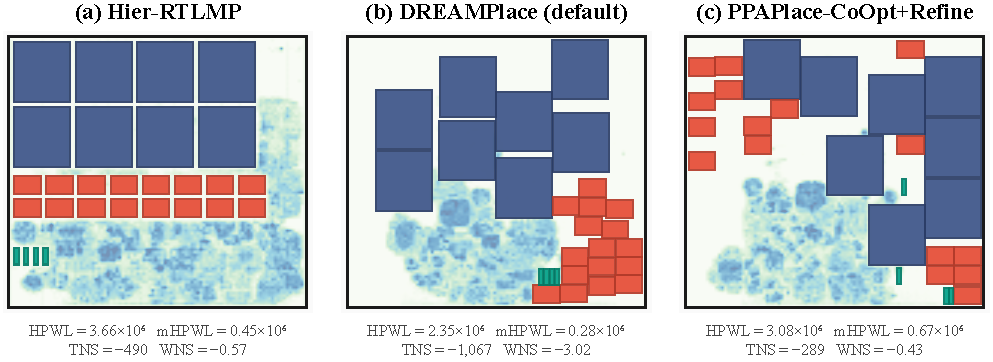
\includegraphics[width=\columnwidth]{graphs/placement_comparison.pdf}
    \caption{Placement comparison on \texttt{swerv\_wrapper}:
    (a)~Hier-RTLMP, (b)~DREAMPlace, (c)~PPAPlace-CoOpt{+}Refine.}
    \label{fig:placement}
\end{figure}

PPAPlace-Refine alone applies gradient descent to DREAMPlace's default
placement, reducing average WNS from $1.61$ to $1.30$ and TNS from
$1.92$ to $1.36$. This improves over untuned DREAMPlace but the
local nature of gradient refinement limits gains on circuits where the
starting topology is already misaligned (ariane133 WNS remains
$2.15\times$).

PPAPlace-CoOpt injects the surrogate co-objective into DREAMPlace's
loop, achieving average WNS of $0.83$ and TNS of $0.57$. The
gap over DREAMPlace\,4.0 demonstrates the value of post-route
supervision over pre-route STA. Post-DRT reports confirm zero design-rule-check
violations and routed wirelength within $3\%$ of default, so the
co-objective does not degrade routability.

Adding Refine after CoOpt further improves average WNS to $0.78$ and
TNS to $0.49$, reaching 22\% and 51\% over Hier-RTLMP. This
surpasses Re$^2$MaP's algorithmic approach ($0.89$/$0.61$) on both
average metrics, demonstrating that a learned post-route objective
can outperform hand-engineered placement heuristics.
Unlike MaskRegulate's circuit-specific gains, CoOpt{+}Refine improves
consistently across all test circuits
(Figure~\ref{fig:main}(a)). It achieves the best per-circuit result
on 6 of 10 circuit--metric pairs and the best average on both WNS
and TNS. On the remaining four pairs, it yields the second-best result
except for the TNS of black\_parrot. The power ratios ($0.99$--$1.02\times$) confirm that PPAPlace's timing improvements do not come at the expense of power performance.  All PPAPlace configurations complete placement in under one minute of wall-clock time.

All the results reported in Table~\ref{tab:main} are final post-DRT PPA metrics. Although the surrogate is trained on post-GRT labels, the improvements carry
through to full detailed routing. This is consistent with the fidelity
analysis in Section~\ref{sec:label_fidelity}, where post-GRT rankings
preserve post-DRT outcomes with $\bar{\rho}=0.86$.

\begin{figure}[h]
    \centering
    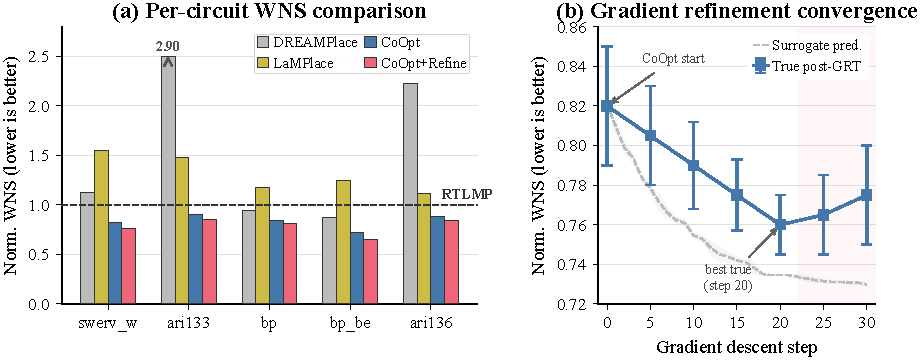
\includegraphics[width=\columnwidth]{graphs/results_main.pdf}
    \caption{(a)~Per-circuit normalized WNS (Table~\ref{tab:main}).
    (b)~True vs.\ surrogate WNS during gradient refinement on swerv\_wrapper.}
    \label{fig:main}
\end{figure}

\subsection{Gradient Quality}
\label{subsec:gradient_quality}

Gradient-guided placement requires directionally accurate gradients.
\texttt{torch.autograd.gradcheck} confirms numerical correctness
(relative error $< 10^{-6}$) on 30 test placements. To assess
directional alignment, we perturb converged placements along 100
random directions per circuit and measure true PPA change via
post-GRT. Table~\ref{tab:gradient_quality} reports cosine similarity
between surrogate and true gradients: average $0.53$ for WNS and
$0.46$ for TNS, positive on all circuits.

\begin{table}[h]
\centering
\caption{Cosine similarity between surrogate gradient and true post-GRT PPA change (100 perturbation directions per circuit).}
\label{tab:gradient_quality}
\renewcommand{\arraystretch}{1.15}
\footnotesize
\begin{tabular}{@{}l cc@{}}
\toprule
Circuit & cos($\nabla$\,WNS) & cos($\nabla$\,TNS) \\
\midrule
swerv\_wrap   & 0.49 & 0.43 \\
ariane133     & 0.58 & 0.49 \\
black\_parrot & 0.51 & 0.46 \\
bp\_be        & 0.62 & 0.53 \\
ariane136     & 0.43 & 0.37 \\
\midrule
Average       & 0.53 & 0.46 \\
\bottomrule
\end{tabular}
\renewcommand{\arraystretch}{1.0}
\end{table}

Figure~\ref{fig:main}(b) validates this on swerv\_wrapper: gradient
descent reduces true post-GRT WNS from $0.82$ to $0.76$ over 20
steps, closely tracked by the surrogate. Beyond step~22, true WNS
rises as the placement exits the training distribution. The
refinement loop retains the best-loss checkpoint across all $T$
steps, so moderate overshoot does not degrade the final result.

We sweep $\lambda_p \in \{0.001, 0.005, 0.01, 0.05\}$ on
swerv\_wrapper, yielding WNS of $\{0.92, 0.87, 0.82, 0.90\}$;
$\lambda_p = 0.01$ provides the best trade-off and is reused
unchanged across all test circuits.
For refinement steps, $T \in \{10, 20, 30, 50\}$ gives WNS
$\{0.79, 0.77, 0.76, 0.77\}$, plateauing at $T{=}30$ before
out-of-distribution degradation begins (Figure~\ref{fig:main}(b)).
The learning rate $\alpha{=}0.001$ is selected by grid search.

\subsection{Generalization}
\label{subsec:generalization}

Table~\ref{tab:generalization} (left) reports ranking accuracy on 500
unseen DREAMPlace placements per test circuit. Average Spearman
$\rho = 0.77$ and Kendall $\tau = 0.58$ for WNS, with top-5 accuracy
of 68\% (vs.\ 2\% for random selection). Accuracy is highest on
bp\_be ($\rho = 0.83$) and lowest on ariane136 ($\rho = 0.72$).
Three test circuits share lineage with training circuits
(bp\_be/bp\_be12, swerv\_wrapper/swerv\_wrapper43, black\_parrot/bp\_fe),
which may inflate their accuracy; ariane133 and ariane136 have no
training-set relatives and indeed show the lowest $\rho$.

\begin{table}[h]
\centering
\caption{Surrogate generalization: ranking accuracy on held-out placements (left) and cross-placer transfer to RTLMP (right).}
\label{tab:generalization}
\renewcommand{\arraystretch}{1.15}
\footnotesize
\begin{tabular}{@{}l ccc cc@{}}
\toprule
& \multicolumn{3}{c}{Held-out (DREAMPlace)}
& \multicolumn{2}{c}{Cross-placer (RTLMP)} \\
\cmidrule(lr){2-4}\cmidrule(lr){5-6}
Circuit & $\rho$ & $\tau$ & Top-5
  & $\rho_\text{WNS}$ & $\rho_\text{TNS}$ \\
\midrule
swerv\_wrap   & 0.74 & 0.56 & 60\% & 0.63 & 0.57 \\
ariane133     & 0.81 & 0.62 & 80\% & 0.58 & 0.54 \\
black\_parrot & 0.77 & 0.55 & 60\% & 0.60 & 0.53 \\
bp\_be        & 0.83 & 0.65 & 80\% & 0.72 & 0.66 \\
ariane136     & 0.72 & 0.51 & 60\% & 0.54 & 0.50 \\
\cmidrule(lr){1-1}\cmidrule(lr){5-6}
bp\_fe\textsuperscript{t}  &  &  &  & 0.68 & 0.60 \\
ethernet\textsuperscript{t}&  &  &  & 0.55 & 0.52 \\
\midrule
Average       & 0.77 & 0.58 & 68\% & 0.61 & 0.56 \\
\bottomrule
\multicolumn{6}{@{}l}{\scriptsize\textsuperscript{t}Training circuit (cross-placer only).}
\end{tabular}
\renewcommand{\arraystretch}{1.0}
\end{table}

Leave-one-circuit-out (LOCO) cross-validation (Figure~\ref{fig:analysis}(a)) trains on
9 circuits and evaluates on the held-out circuit. Per-circuit $\tau$
ranges from $0.07$ (isa\_npu) to $0.28$ (mor1kx), modest individually
but sufficient for the surrogate to consistently identify
above-average placements in deployment.

\begin{figure}[h]
    \centering
    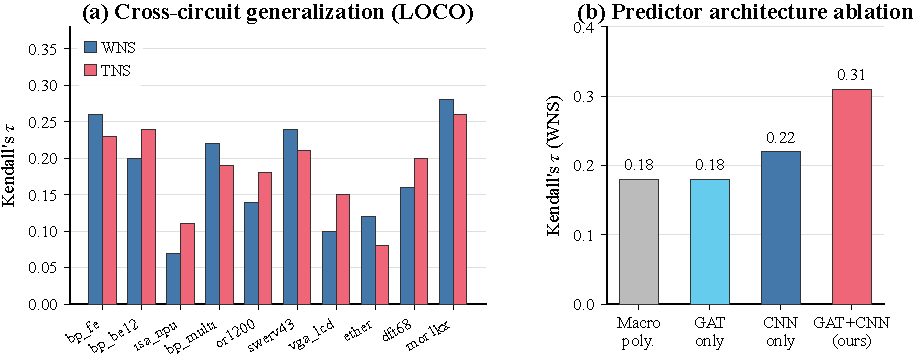
\includegraphics[width=\columnwidth]{graphs/results_analysis.pdf}
    \caption{(a)~Leave-one-circuit-out (LOCO) cross-circuit generalization (Kendall's $\tau$).
    (b)~Predictor architecture ablation (Kendall's $\tau$).}
    \label{fig:analysis}
\end{figure}

Table~\ref{tab:generalization} (right) applies the DREAMPlace-trained
predictor to RTLMP configurations. The predictor has never seen RTLMP
placements during training. Cross-placer $\rho$ averages 0.61 for
WNS, lower than within-placer (0.77) but statistically significant
($p < 0.01$) on all tested circuits. This confirms that the surrogate
learns physical patterns that transfer across placement paradigms.


\subsection{Ablation Studies}
\label{subsec:ablations}

\begin{table}[t]
\centering
\caption{Ablation on labels and representation (Kendall's $\tau$, WNS). Upper: $2 \times 2$ factorial; lower: label stage progression.}
\label{tab:ablation_combined}
\renewcommand{\arraystretch}{1.15}
\footnotesize
\begin{tabular}{@{}ll cc@{}}
\toprule
Training labels & Architecture & $\tau$ (WNS) & Top-1 \\
\midrule
\multicolumn{4}{@{}l}{\emph{Label $\times$ representation}} \\[1pt]
Pre-route STA & Macro-only poly.\ & 0.08\tpm.02 & n/a \\
Pre-route STA & GAT+CNN & 0.13\tpm.03 & 26\% \\
Post-GRT      & Macro-only poly.\ & 0.18\tpm.02 & n/a \\
Post-GRT      & GAT+CNN & \textbf{0.31\tpm.02} & \textbf{52\%} \\
\midrule
\multicolumn{4}{@{}l}{\emph{Label stage (GAT+CNN fixed)}} \\[1pt]
Post-CTS      & GAT+CNN & 0.16\tpm.03 & 30\% \\
Post-DRT      & GAT+CNN & 0.34\tpm.02 & 56\% \\
\bottomrule
\end{tabular}
\renewcommand{\arraystretch}{1.0}
\end{table}

\subsubsection{Label Fidelity and Representation}
\label{subsec:2x2}

The upper section of Table~\ref{tab:ablation_combined} crosses two
label stages with two representations under identical training. The macro-only + pre-route STA cell ($\tau = 0.08$), which
corresponds to LaMPlace's design choices, is barely above random. Both axes contribute
independently. Post-GRT labels double macro-only $\tau$ from 0.08 to
0.18. The GAT+CNN representation raises pre-route $\tau$ from 0.08 to
0.13. The combined setting (mixed-size + post-GRT) reaches
$\tau = 0.31$.

The lower section isolates the label axis with a fixed GAT+CNN
architecture. Post-CTS ($\tau = 0.16$) yields near-random ranking.
Post-GRT ($\tau = 0.31$) roughly doubles the correlation. Post-DRT
provides a modest further gain ($\tau = 0.34$) at $6\times$ the
labeling cost. Under a fixed 48-hour budget, 500 post-GRT samples
($\tau = 0.31$) outperform 80 post-DRT samples ($\tau = 0.28$),
confirming that the additional data volume from cheaper labels more
than compensates for the slight fidelity gap.

\subsubsection{Predictor Architecture}
\label{subsec:pred_results}

The $2 \times 2$ experiment established that the mixed-size
representation matters. Figure~\ref{fig:analysis}(b) unpacks which
components contribute. Four variants are compared, all trained on
post-GRT labels: macro-only polynomial ($\tau = 0.18$), CNN-only
($\tau = 0.22$), GAT-only ($\tau = 0.18$), and GAT+CNN
($\tau = 0.31$). The spatial stream alone outperforms the graph
stream alone. Their combination exceeds either single stream,
indicating that density patterns and connectivity structure provide
complementary information.


%% ============================================================
\section{Conclusion}
\label{sec:conclusion}

PPAPlace demonstrates that a differentiable surrogate trained on
post-GRT labels can provide gradient-based PPA feedback that no
analytical proxy achieves. CoOpt{+}Refine improves average WNS and
TNS by 22\% and 51\% over Hier-RTLMP on five unseen circuits.

Despite the performance gains, several limitations suggest promising future directions. The surrogate is trained on the Nangate45 library only. Validating
generalization across technology nodes and standard-cell libraries is
a natural next step, requiring only regeneration of the post-GRT
labeling pipeline. Gradient refinement exhibits out-of-distribution
degradation beyond 20 steps (Figure~\ref{fig:main}(b)).
Distribution-aware stopping or trust-region constraints could improve
robustness. Cross-placer transfer ($\rho = 0.61$) lags behind
within-placer accuracy ($0.77$). Targeted fine-tuning or
domain-adaptation techniques could narrow this gap. Finally, CoOpt
currently requires integration with a differentiable placer.
Extending the co-objective paradigm to commercial tools that expose
only final placements remains an open challenge that the
placer-agnostic Refine mode partially addresses.

 
%% ============================================================
\newpage
\bibliographystyle{ACM-Reference-Format}
\bibliography{references}

\end{document}